\documentclass[twoside]{book}

% Packages required by doxygen
\usepackage{fixltx2e}
\usepackage{calc}
\usepackage{doxygen}
\usepackage[export]{adjustbox} % also loads graphicx
\usepackage{graphicx}
\usepackage[utf8]{inputenc}
\usepackage{makeidx}
\usepackage{multicol}
\usepackage{multirow}
\PassOptionsToPackage{warn}{textcomp}
\usepackage{textcomp}
\usepackage[nointegrals]{wasysym}
\usepackage[table]{xcolor}

% Font selection
\usepackage[T1]{fontenc}
\usepackage[scaled=.90]{helvet}
\usepackage{courier}
\usepackage{amssymb}
\usepackage{sectsty}
\renewcommand{\familydefault}{\sfdefault}
\allsectionsfont{%
  \fontseries{bc}\selectfont%
  \color{darkgray}%
}
\renewcommand{\DoxyLabelFont}{%
  \fontseries{bc}\selectfont%
  \color{darkgray}%
}
\newcommand{\+}{\discretionary{\mbox{\scriptsize$\hookleftarrow$}}{}{}}

% Page & text layout
\usepackage{geometry}
\geometry{%
  a4paper,%
  top=2.5cm,%
  bottom=2.5cm,%
  left=2.5cm,%
  right=2.5cm%
}
\tolerance=750
\hfuzz=15pt
\hbadness=750
\setlength{\emergencystretch}{15pt}
\setlength{\parindent}{0cm}
\setlength{\parskip}{3ex plus 2ex minus 2ex}
\makeatletter
\renewcommand{\paragraph}{%
  \@startsection{paragraph}{4}{0ex}{-1.0ex}{1.0ex}{%
    \normalfont\normalsize\bfseries\SS@parafont%
  }%
}
\renewcommand{\subparagraph}{%
  \@startsection{subparagraph}{5}{0ex}{-1.0ex}{1.0ex}{%
    \normalfont\normalsize\bfseries\SS@subparafont%
  }%
}
\makeatother

% Headers & footers
\usepackage{fancyhdr}
\pagestyle{fancyplain}
\fancyhead[LE]{\fancyplain{}{\bfseries\thepage}}
\fancyhead[CE]{\fancyplain{}{}}
\fancyhead[RE]{\fancyplain{}{\bfseries\leftmark}}
\fancyhead[LO]{\fancyplain{}{\bfseries\rightmark}}
\fancyhead[CO]{\fancyplain{}{}}
\fancyhead[RO]{\fancyplain{}{\bfseries\thepage}}
\fancyfoot[LE]{\fancyplain{}{}}
\fancyfoot[CE]{\fancyplain{}{}}
\fancyfoot[RE]{\fancyplain{}{\bfseries\scriptsize Generated by Doxygen }}
\fancyfoot[LO]{\fancyplain{}{\bfseries\scriptsize Generated by Doxygen }}
\fancyfoot[CO]{\fancyplain{}{}}
\fancyfoot[RO]{\fancyplain{}{}}
\renewcommand{\footrulewidth}{0.4pt}
\renewcommand{\chaptermark}[1]{%
  \markboth{#1}{}%
}
\renewcommand{\sectionmark}[1]{%
  \markright{\thesection\ #1}%
}

% Indices & bibliography
\usepackage{natbib}
\usepackage[titles]{tocloft}
\setcounter{tocdepth}{3}
\setcounter{secnumdepth}{5}
\makeindex

% Hyperlinks (required, but should be loaded last)
\usepackage{ifpdf}
\ifpdf
  \usepackage[pdftex,pagebackref=true]{hyperref}
\else
  \usepackage[ps2pdf,pagebackref=true]{hyperref}
\fi
\hypersetup{%
  colorlinks=true,%
  linkcolor=blue,%
  citecolor=blue,%
  unicode%
}

% Custom commands
\newcommand{\clearemptydoublepage}{%
  \newpage{\pagestyle{empty}\cleardoublepage}%
}

\usepackage{caption}
\captionsetup{labelsep=space,justification=centering,font={bf},singlelinecheck=off,skip=4pt,position=top}

%===== C O N T E N T S =====

\usepackage{CJKutf8}
\begin {document}
\begin{CJK}{UTF8}{gbsn}


% Titlepage & ToC
\hypersetup{pageanchor=false,
             bookmarksnumbered=true,
             pdfencoding=unicode
            }
\pagenumbering{roman}
\begin{titlepage}
\vspace*{7cm}
\begin{center}%
{\Large My Project }\\
\vspace*{1cm}
{\large Generated by Doxygen 1.8.11}\\
\end{center}
\end{titlepage}
\clearemptydoublepage
\tableofcontents
\clearemptydoublepage
\pagenumbering{arabic}
\hypersetup{pageanchor=true}

%--- Begin generated contents ---
\chapter{Class Index}
\section{Class List}
Here are the classes, structs, unions and interfaces with brief descriptions\+:\begin{DoxyCompactList}
\item\contentsline{section}{\hyperlink{classhw3}{hw3} }{\pageref{classhw3}}{}
\end{DoxyCompactList}

\chapter{File Index}
\section{File List}
Here is a list of all documented files with brief descriptions\+:\begin{DoxyCompactList}
\item\contentsline{section}{\hyperlink{hw3_8cpp}{hw3.\+cpp} \\*函数实现 }{\pageref{hw3_8cpp}}{}
\item\contentsline{section}{\hyperlink{hw3_8h}{hw3.\+h} }{\pageref{hw3_8h}}{}
\item\contentsline{section}{\hyperlink{main_8cpp}{main.\+cpp} }{\pageref{main_8cpp}}{}
\end{DoxyCompactList}

\chapter{Class Documentation}
\hypertarget{classHeat}{}\section{Heat Class Reference}
\label{classHeat}\index{Heat@{Heat}}
\subsection*{Public Member Functions}
\begin{DoxyCompactItemize}
\item 
void \hyperlink{classHeat_abea1c1c77c8fd8654c9cdef12a238eeb}{set\+\_\+size} (int)
\begin{DoxyCompactList}\small\item\em 设置进程总数 \end{DoxyCompactList}\item 
void \hyperlink{classHeat_a95a5f94ca3965c0ba13ea1258eea31e4}{set\+\_\+rank} (int)
\begin{DoxyCompactList}\small\item\em 设置进程编号 \end{DoxyCompactList}\item 
void \hyperlink{classHeat_a3b7d978b4d27645c6f6bacd55c8cdbc2}{set\+\_\+f} (const R\+HS \&)
\begin{DoxyCompactList}\small\item\em 设置右端项f \end{DoxyCompactList}\item 
void \hyperlink{classHeat_a7dbbbb774cb0317d18a31342ce8e6865}{set\+\_\+\+Initial} (const R\+HF \&)
\begin{DoxyCompactList}\small\item\em 设置初值 \end{DoxyCompactList}\item 
void \hyperlink{classHeat_a5277a27b4f971ed54e66d8fe8ffe97f7}{set\+\_\+\+Boundrary} (int, const R\+HS \&)
\begin{DoxyCompactList}\small\item\em 设置边值 \end{DoxyCompactList}\item 
void \hyperlink{classHeat_af7b0ad84d2b149a944bada144c3e450f}{set\+\_\+N} (int)
\begin{DoxyCompactList}\small\item\em 设置网格密度 \end{DoxyCompactList}\item 
void \hyperlink{classHeat_a890e689eed8ad3992ff8b50dae40cace}{set\+\_\+t} (double)
\begin{DoxyCompactList}\small\item\em 设置计算终止时间 \end{DoxyCompactList}\item 
void \hyperlink{classHeat_ad50289d77a5715fa1aa63af60956ae26}{set\+\_\+\+C\+FL} (double)
\begin{DoxyCompactList}\small\item\em 设置\+C\+F\+L条件数 \end{DoxyCompactList}\item 
void \hyperlink{classHeat_af702ba3e9068a9b680e72a2e83591a48}{set\+\_\+\+Solution} (const R\+HS \&)
\begin{DoxyCompactList}\small\item\em 设置真解,可以用来对有真解的情况测试误差. \end{DoxyCompactList}\item 
double \hyperlink{classHeat_af454cb46d03902ab4fd2ec5aa1169786}{error} ()
\begin{DoxyCompactList}\small\item\em 计算误差的一个测试函数 \end{DoxyCompactList}\item 
std\+::vector$<$ double $>$ \hyperlink{classHeat_af166af7cfc6e7a3118ac97be84c0c75b}{solve} ()
\begin{DoxyCompactList}\small\item\em 求解函数 \end{DoxyCompactList}\end{DoxyCompactItemize}


\subsection{Member Function Documentation}
\index{Heat@{Heat}!error@{error}}
\index{error@{error}!Heat@{Heat}}
\subsubsection[{\texorpdfstring{error()}{error()}}]{\setlength{\rightskip}{0pt plus 5cm}double Heat\+::error (
\begin{DoxyParamCaption}
{}
\end{DoxyParamCaption}
)}\hypertarget{classHeat_af454cb46d03902ab4fd2ec5aa1169786}{}\label{classHeat_af454cb46d03902ab4fd2ec5aa1169786}


计算误差的一个测试函数 

\begin{DoxyReturn}{Returns}
L2误差 
\end{DoxyReturn}
\index{Heat@{Heat}!set\+\_\+\+Boundrary@{set\+\_\+\+Boundrary}}
\index{set\+\_\+\+Boundrary@{set\+\_\+\+Boundrary}!Heat@{Heat}}
\subsubsection[{\texorpdfstring{set\+\_\+\+Boundrary(int, const R\+H\+S \&)}{set_Boundrary(int, const RHS &)}}]{\setlength{\rightskip}{0pt plus 5cm}void Heat\+::set\+\_\+\+Boundrary (
\begin{DoxyParamCaption}
\item[{int}]{flag, }
\item[{const R\+HS \&}]{fun}
\end{DoxyParamCaption}
)}\hypertarget{classHeat_a5277a27b4f971ed54e66d8fe8ffe97f7}{}\label{classHeat_a5277a27b4f971ed54e66d8fe8ffe97f7}


设置边值 


\begin{DoxyParams}{Parameters}
{\em flag} & 标志, D\+I\+R\+I\+C\+H\+L\+ET 或者 N\+E\+U\+M\+A\+NN \\
\hline
{\em fun} & \\
\hline
\end{DoxyParams}
\index{Heat@{Heat}!set\+\_\+\+C\+FL@{set\+\_\+\+C\+FL}}
\index{set\+\_\+\+C\+FL@{set\+\_\+\+C\+FL}!Heat@{Heat}}
\subsubsection[{\texorpdfstring{set\+\_\+\+C\+F\+L(double)}{set_CFL(double)}}]{\setlength{\rightskip}{0pt plus 5cm}void Heat\+::set\+\_\+\+C\+FL (
\begin{DoxyParamCaption}
\item[{double}]{C\+F\+L1}
\end{DoxyParamCaption}
)}\hypertarget{classHeat_ad50289d77a5715fa1aa63af60956ae26}{}\label{classHeat_ad50289d77a5715fa1aa63af60956ae26}


设置\+C\+F\+L条件数 


\begin{DoxyParams}{Parameters}
{\em C\+F\+L1} & \\
\hline
\end{DoxyParams}
\index{Heat@{Heat}!set\+\_\+f@{set\+\_\+f}}
\index{set\+\_\+f@{set\+\_\+f}!Heat@{Heat}}
\subsubsection[{\texorpdfstring{set\+\_\+f(const R\+H\+S \&)}{set_f(const RHS &)}}]{\setlength{\rightskip}{0pt plus 5cm}void Heat\+::set\+\_\+f (
\begin{DoxyParamCaption}
\item[{const R\+HS \&}]{fun}
\end{DoxyParamCaption}
)}\hypertarget{classHeat_a3b7d978b4d27645c6f6bacd55c8cdbc2}{}\label{classHeat_a3b7d978b4d27645c6f6bacd55c8cdbc2}


设置右端项f 


\begin{DoxyParams}{Parameters}
{\em fun} & \\
\hline
\end{DoxyParams}
\index{Heat@{Heat}!set\+\_\+\+Initial@{set\+\_\+\+Initial}}
\index{set\+\_\+\+Initial@{set\+\_\+\+Initial}!Heat@{Heat}}
\subsubsection[{\texorpdfstring{set\+\_\+\+Initial(const R\+H\+F \&)}{set_Initial(const RHF &)}}]{\setlength{\rightskip}{0pt plus 5cm}void Heat\+::set\+\_\+\+Initial (
\begin{DoxyParamCaption}
\item[{const R\+HF \&}]{fun}
\end{DoxyParamCaption}
)}\hypertarget{classHeat_a7dbbbb774cb0317d18a31342ce8e6865}{}\label{classHeat_a7dbbbb774cb0317d18a31342ce8e6865}


设置初值 


\begin{DoxyParams}{Parameters}
{\em fun} & \\
\hline
\end{DoxyParams}
\index{Heat@{Heat}!set\+\_\+N@{set\+\_\+N}}
\index{set\+\_\+N@{set\+\_\+N}!Heat@{Heat}}
\subsubsection[{\texorpdfstring{set\+\_\+\+N(int)}{set_N(int)}}]{\setlength{\rightskip}{0pt plus 5cm}void Heat\+::set\+\_\+N (
\begin{DoxyParamCaption}
\item[{int}]{N1}
\end{DoxyParamCaption}
)}\hypertarget{classHeat_af7b0ad84d2b149a944bada144c3e450f}{}\label{classHeat_af7b0ad84d2b149a944bada144c3e450f}


设置网格密度 


\begin{DoxyParams}{Parameters}
{\em N1} & \\
\hline
\end{DoxyParams}
\index{Heat@{Heat}!set\+\_\+rank@{set\+\_\+rank}}
\index{set\+\_\+rank@{set\+\_\+rank}!Heat@{Heat}}
\subsubsection[{\texorpdfstring{set\+\_\+rank(int)}{set_rank(int)}}]{\setlength{\rightskip}{0pt plus 5cm}void Heat\+::set\+\_\+rank (
\begin{DoxyParamCaption}
\item[{int}]{rank1}
\end{DoxyParamCaption}
)}\hypertarget{classHeat_a95a5f94ca3965c0ba13ea1258eea31e4}{}\label{classHeat_a95a5f94ca3965c0ba13ea1258eea31e4}


设置进程编号 


\begin{DoxyParams}{Parameters}
{\em rank1} & \\
\hline
\end{DoxyParams}
\index{Heat@{Heat}!set\+\_\+size@{set\+\_\+size}}
\index{set\+\_\+size@{set\+\_\+size}!Heat@{Heat}}
\subsubsection[{\texorpdfstring{set\+\_\+size(int)}{set_size(int)}}]{\setlength{\rightskip}{0pt plus 5cm}void Heat\+::set\+\_\+size (
\begin{DoxyParamCaption}
\item[{int}]{size1}
\end{DoxyParamCaption}
)}\hypertarget{classHeat_abea1c1c77c8fd8654c9cdef12a238eeb}{}\label{classHeat_abea1c1c77c8fd8654c9cdef12a238eeb}


设置进程总数 


\begin{DoxyParams}{Parameters}
{\em size1} & \\
\hline
\end{DoxyParams}
\index{Heat@{Heat}!set\+\_\+\+Solution@{set\+\_\+\+Solution}}
\index{set\+\_\+\+Solution@{set\+\_\+\+Solution}!Heat@{Heat}}
\subsubsection[{\texorpdfstring{set\+\_\+\+Solution(const R\+H\+S \&)}{set_Solution(const RHS &)}}]{\setlength{\rightskip}{0pt plus 5cm}void Heat\+::set\+\_\+\+Solution (
\begin{DoxyParamCaption}
\item[{const R\+HS \&}]{uu}
\end{DoxyParamCaption}
)}\hypertarget{classHeat_af702ba3e9068a9b680e72a2e83591a48}{}\label{classHeat_af702ba3e9068a9b680e72a2e83591a48}


设置真解,可以用来对有真解的情况测试误差. 


\begin{DoxyParams}{Parameters}
{\em uu} & \\
\hline
\end{DoxyParams}
\index{Heat@{Heat}!set\+\_\+t@{set\+\_\+t}}
\index{set\+\_\+t@{set\+\_\+t}!Heat@{Heat}}
\subsubsection[{\texorpdfstring{set\+\_\+t(double)}{set_t(double)}}]{\setlength{\rightskip}{0pt plus 5cm}void Heat\+::set\+\_\+t (
\begin{DoxyParamCaption}
\item[{double}]{t1}
\end{DoxyParamCaption}
)}\hypertarget{classHeat_a890e689eed8ad3992ff8b50dae40cace}{}\label{classHeat_a890e689eed8ad3992ff8b50dae40cace}


设置计算终止时间 


\begin{DoxyParams}{Parameters}
{\em t1} & \\
\hline
\end{DoxyParams}
\index{Heat@{Heat}!solve@{solve}}
\index{solve@{solve}!Heat@{Heat}}
\subsubsection[{\texorpdfstring{solve()}{solve()}}]{\setlength{\rightskip}{0pt plus 5cm}std\+::vector$<$ double $>$ Heat\+::solve (
\begin{DoxyParamCaption}
{}
\end{DoxyParamCaption}
)}\hypertarget{classHeat_af166af7cfc6e7a3118ac97be84c0c75b}{}\label{classHeat_af166af7cfc6e7a3118ac97be84c0c75b}


求解函数 

\begin{DoxyReturn}{Returns}
0号进程返回整个解,其余进程返回各自负责的区域的解。 
\end{DoxyReturn}


The documentation for this class was generated from the following files\+:\begin{DoxyCompactItemize}
\item 
\hyperlink{Heat_8h}{Heat.\+h}\item 
\hyperlink{Heat_8cpp}{Heat.\+cpp}\end{DoxyCompactItemize}

\chapter{File Documentation}
\hypertarget{Heat_8cpp}{}\section{Heat.\+cpp File Reference}
\label{Heat_8cpp}\index{Heat.\+cpp@{Heat.\+cpp}}
{\ttfamily \#include \char`\"{}Heat.\+h\char`\"{}}\\*
Include dependency graph for Heat.\+cpp\+:

\hypertarget{Heat_8h}{}\section{Heat.\+h File Reference}
\label{Heat_8h}\index{Heat.\+h@{Heat.\+h}}
{\ttfamily \#include $<$iostream$>$}\\*
{\ttfamily \#include $<$vector$>$}\\*
{\ttfamily \#include $<$cmath$>$}\\*
{\ttfamily \#include $<$cstdlib$>$}\\*
{\ttfamily \#include \char`\"{}mpi.\+h\char`\"{}}\\*
Include dependency graph for Heat.\+h\+:
% FIG 0
This graph shows which files directly or indirectly include this file\+:
% FIG 1
\subsection*{Classes}
\begin{DoxyCompactItemize}
\item 
class \hyperlink{classHeat}{Heat}
\end{DoxyCompactItemize}
\subsection*{Enumerations}
\begin{DoxyCompactItemize}
\item 
enum \{ {\bfseries D\+I\+R\+I\+C\+H\+L\+ET} = 1, 
{\bfseries N\+E\+U\+M\+A\+NN} = 2
 \}\hypertarget{Heat_8h_a06fc87d81c62e9abb8790b6e5713c55b}{}\label{Heat_8h_a06fc87d81c62e9abb8790b6e5713c55b}

\end{DoxyCompactItemize}


\subsection{Detailed Description}
\begin{DoxyAuthor}{Author}
lczheng, \href{mailto:lczheng@pku.edu.cn}{\tt lczheng@pku.\+edu.\+cn}
\end{DoxyAuthor}
\begin{DoxyDate}{Date}
2016-\/11-\/08 
\end{DoxyDate}

\hypertarget{main_8cpp}{}\section{main.\+cpp File Reference}
\label{main_8cpp}\index{main.\+cpp@{main.\+cpp}}
{\ttfamily \#include \char`\"{}Heat.\+h\char`\"{}}\\*
Include dependency graph for main.\+cpp\+:
\nopagebreak
\begin{figure}[H]
\begin{center}
\leavevmode
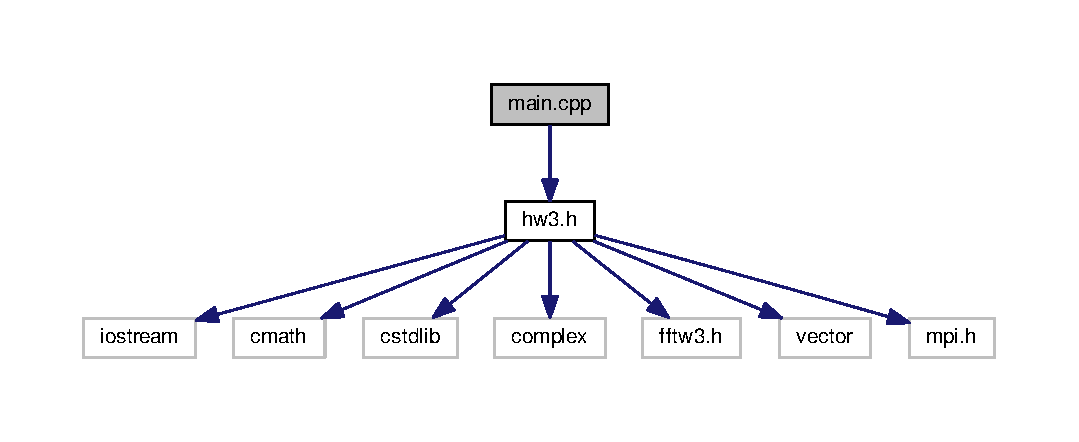
\includegraphics[width=350pt]{main_8cpp__incl}
\end{center}
\end{figure}
\subsection*{Functions}
\begin{DoxyCompactItemize}
\item 
double {\bfseries u} (double x, double y, double z, double t)\hypertarget{main_8cpp_a7f946b7182f074fdec4cd02cceec0f95}{}\label{main_8cpp_a7f946b7182f074fdec4cd02cceec0f95}

\item 
double {\bfseries f} (double x, double y, double z, double t)\hypertarget{main_8cpp_a2cb048afa8f6f33ffe18db917a6164b0}{}\label{main_8cpp_a2cb048afa8f6f33ffe18db917a6164b0}

\item 
double {\bfseries u0} (double x, double y, double z)\hypertarget{main_8cpp_a50b8caccf6e7fea0ad0cf221da153050}{}\label{main_8cpp_a50b8caccf6e7fea0ad0cf221da153050}

\item 
double {\bfseries g\+\_\+up} (double x, double y, double z, double t)\hypertarget{main_8cpp_a24122920a607797e7ee374ea86e07f26}{}\label{main_8cpp_a24122920a607797e7ee374ea86e07f26}

\item 
double {\bfseries g\+\_\+down} (double x, double y, double z, double t)\hypertarget{main_8cpp_a76d374eeb92bbd16ef04a38748906749}{}\label{main_8cpp_a76d374eeb92bbd16ef04a38748906749}

\item 
int {\bfseries transform} (int i, int j, int k, int N)\hypertarget{main_8cpp_a2ea6b0858e6766287931140dcb973820}{}\label{main_8cpp_a2ea6b0858e6766287931140dcb973820}

\item 
int {\bfseries main} (int argc, char $\ast$argv\mbox{[}$\,$\mbox{]})\hypertarget{main_8cpp_a0ddf1224851353fc92bfbff6f499fa97}{}\label{main_8cpp_a0ddf1224851353fc92bfbff6f499fa97}

\end{DoxyCompactItemize}


\subsection{Detailed Description}
\begin{DoxyAuthor}{Author}
lczheng, \href{mailto:lczheng@pku.edu.cn}{\tt lczheng@pku.\+edu.\+cn}
\end{DoxyAuthor}
\begin{DoxyDate}{Date}
2016-\/12-\/31 
\end{DoxyDate}

%--- End generated contents ---

% Index
\backmatter
\newpage
\phantomsection
\clearemptydoublepage
\addcontentsline{toc}{chapter}{Index}
\printindex

\end{CJK}
\end {document}
